%% =======================================================================================
%% 
%% RELATÓRIO TÉCNICO
%% Criado a partir da classe abntex2, desenvolvida pelo 
%% Centro de Pesquisa em Arquitetura da Informação (CPAI)
%% 
%% Arquivos de dados:   sty/configs.sty         % Configuração dos pacotes LaTeX
%%                      sty/metadados_rt.sty    % METADADOS DO RELATÓRIO - PREENCHER!
%%                      sty/dados_cpai.sty      % Informações institucionais CPAI / FUB
%%                      sty/timbrado.sty        % Formatação do documento (layout)
%%                      sty/vocabulario.sty     % Comandos LaTeX para facilitar digitação
%% 
%% =======================================================================================

\documentclass[pdftex,12pt,oneside,a4paper,english,french,spanish,brazil]{abntex2}


% ----------------------------------------------------------------------------------------
% - PACOTES
  \usepackage{sty/configs}                  % Pacotes utilizados
  \usepackage{sty/metadados_rt}             % Dados do órgão / cliente
  \usepackage{sty/dados_cpai}               % Dados do CPAI/FUB
  \usepackage{sty/vocabulario}              % Vocabulário específico do projeto
  \usepackage{sty/leiaute_rt}               % Definições de layout do documento

% ----------------------------------------------------------------------------------------

% ----------------------------------------------------------------------------------------
% - INÍCIO DO DOCUMENTO
  \begin{document}
      \begin{sloppypar}
          
          % Seleciona o idioma do documento (conforme pacotes do babel)
            %\selectlanguage{english}
            \selectlanguage{brazil}
            
          % Retira espaço extra obsoleto entre as frases.
            \frenchspacing
          
          % ------------------------------------------------------------------------------
          % - ESTRUTURA DO DOCUMENTO
          % ------------------------------------------------------------------------------
          % ------------------------------------------------------------------------------
          % - PRÉ-TEXTUAL
          % ------------------------------------------------------------------------------
          \pretextual

          % Capa
            %~~~~~~~~~~~~~~~~~~~~~~~~~~~~~~~~~~~~~~~~~~~~~~~~~~~~~~~~~~~~~~~~~~~~~
% File  : capa
%~~~~~~~~~~~~~~~~~~~~~~~~~~~~~~~~~~~~~~~~~~~~~~~~~~~~~~~~~~~~~~~~~~~~~

% Limpa os estilos de página
  \thispagestyle{empty}

% Desenho no fundo da página
  \ThisCenterWallPaper{1}{img/CapaTR3.pdf}

% Cria uma mini-página para inserir os dados da capa usando 70% da largura do texto
  \begin{flushright}

    \begin{minipage}{0.6\textwidth}
      \begin{flushleft}
          \sffamily
          % Parte superior da capa
          \vspace{2cm}
          \LARGE \textbf{\rttipo} \\
          \footnotesize \textcolor{black!60}{\rtid} \\[2cm]
          \Huge \textbf{\rttitulo} \\
      \end{flushleft}
    \end{minipage}%

    \vfill
    \begin{minipage}{0.6\textwidth}
        \begin{center}
          % Rodapé da capa
          \sffamily
          \small \rtlocal \\
          Versão \rtversao \\
          \rtdata \\
        \end{center}
    \end{minipage}%
  \end{flushright}

            \cleardoublepage
          
          % Revisões
            %~~~~~~~~~~~~~~~~~~~~~~~~~~~~~~~~~~~~~~~~~~~~~~~~~~~~~~~~~~~~~~~~~~~~~
% File  : revisoes
%~~~~~~~~~~~~~~~~~~~~~~~~~~~~~~~~~~~~~~~~~~~~~~~~~~~~~~~~~~~~~~~~~~~~~

% Tabela de revisões do plano de trabalho

{
    %\ABNTEXchapterfont
    \setlength{\parindent}{0cm}
    
    \vspace*{\fill} 
    
    {\sffamily \Large Identificação}

        \begin{tabular}{r p{12cm}}
            \emph{Título:}    & \rttipo: \rttitulo \\
            & {\footnotesize  \textcolor{black!60}{\rtid}} \\
            \emph{Projeto:}   & \rtprojeto \\
            \emph{Data:}      & \rtdata \\
            \emph{Local:}     & \rtlocal \\
            \emph{Versão:}    & \rtversao \\
        \end{tabular}
    
    \vspace{1cm}
    {\sffamily \Large Revisões}

        \begin{footnotesize}
            \begin{tabular}{p{1.8cm}|p{8.5cm}|p{4.5cm}}
                %=============================================================
                % = CABEÇALHO
                \hline
                \textbf{Data} & \textbf{Alterações / Comentário} & \textbf{Revisor} \\ \hline
                %=============================================================
                
                %=============================================================
                % = REVISÕES
                2016.11.14 &
                Criação do documento. &
                Bruno Carvalho C. Souza \\ \hline
                
                %=============================================================
            \end{tabular}
        \end{footnotesize}

}

%----------------------------------------------------------------------
            \cleardoublepage

          % Filiação CPAI
            %~~~~~~~~~~~~~~~~~~~~~~~~~~~~~~~~~~~~~~~~~~~~~~~~~~~~~~~~~~~~~~~~~~~~~
% File  : filiacao_cpai
%~~~~~~~~~~~~~~~~~~~~~~~~~~~~~~~~~~~~~~~~~~~~~~~~~~~~~~~~~~~~~~~~~~~~~

%---------------------------------------------------------------------
{
\ABNTEXchapterfont\setlength{\parindent}{0cm}
\textsf{\textbf{\UnB\ -- UnB} }

{\scriptsize \textsf{\textbf{Reitora}}} \\ % {\tiny (Gestão 2012--2016)}
\textsc{\reitor}

{\scriptsize \textsf{\textbf{Vice-reitor}}}\\
\textsc{\vicereitor}


%---------------------------------------------------------------------
\vspace{0.8cm}

\textsf{\textbf{Centro de Pesquisa em Arquitetura da Informação -- CPAI}}

{\scriptsize \textsf{\textbf{Diretor}}}\\
\textsc{\diretorcpai}

\vfill
\textsf{\textbf{Pesquisador Líder}} \\
\textsc{\rtlider} \\

\textsf{\textbf{Equipe de Pesquisa (em ordem alfabética)}}

%\textsc{Ângelo Henrique Gonçalves Ramim} {\scriptsize (Analista de Tecnologia)} \\
\textsc{Ângelo Henrique Gonçalves Ramim} \\
\textsc{Bruno Carvalho Castro Souza} \\
\textsc{Cláudio Roberto Vieira Chaves} \\
\textsc{Ismael de Moura Costa} \\
\textsc{Lauro César Araujo} \\
\textsc{Mamede Lima-Marques} \\
\textsc{Odilon Neves Júnior} \\
\textsc{Paulo Argolo da Cruz Rios Filho} \\
\textsc{Renan Lima Alves} \\
\textsc{Romualdo Alves Pereira Junior} \\
%\textsc{Carlos Benedito Lima de Menezes} {\scriptsize (Assistente em Administração)} \\
%\textsc{Claudio Monteiro} {\scriptsize (Estagiário Técnico)} \\
%\textsc{Cláudio Roberto Vieira Chaves} {\scriptsize (Analista de Tecnologia)} \\
%\textsc{Deise de Sousa Lima} {\scriptsize (Auxiliar em Administração)} \\
%\textsc{Fabiana de Souza Damatta} {\scriptsize (Administradora)} \\
%\textsc{Jucilene Gomes Moreira} {\scriptsize (Secretária da Diretoria)} \\
%\textsc{Maria das  Dores F. Figueredo} {\scriptsize (Secretária da Diretoria)} \\
%\textsc{Moíses  Lobo de Souza Choas} {\scriptsize (Bolsista / Estagiário)} \\
%\textsc{Paulo Argolo da Cruz Rios Filho} {\scriptsize (Analista de Tecnologia)} \\
%\vspace{1cm}


%{\scriptsize \textsf{\textbf{Vice-diretor}}}\\
%\textsc{Eudes de Queiroz e Silva}

%---------------------------------------------------------------------
%\vspace{0.8cm}

%\textsf{\textbf{Centro de Seleção e de Promoção de Eventos -- CESPE}}

%{\scriptsize \textsf{\textbf{Diretor-Geral}}}\\
%\textsc{Paulo Henrique Portela}

%---------------------------------------------------------------------
%\vspace{0.8cm}

%\textsf{\textbf{Centro de  Documentação -- CEDOC}}

%{\scriptsize \textsf{\textbf{Diretora}}}\\
%\textsc{Cynthia Roncaglio}


}


%---------------------------------------------------------------------
%\clearpage

%\vspace{1cm}

%\textsf{\textbf{Grupo de Trabalho}} \hfill {\scriptsize Resolução da Reitoria n\ele\ 0068/2013}

%\vspace{1cm}

%\textsc{\mlm} -- \cpai\ -- Presidente

%\textsc{Helena Fernandes Guedes Rafael} -- \cpai\

%\textsc{Mauro Henrique de Castro} -- CESPE

%\textsc{Alexandre Schwantz} -- CESPE

%\textsc{Cynthia Roncaglio} -- CEDOC

%\cleardoublepage

%---------------------------------------------------------------------
% Fim de arquivo
%~~~~~~~~~~~~~~~~~~~~~~~~~~~~~~~~~~~~~~~~~~~~~~~~~~~~~~~~~~~~~~~~~~~~~

            \cleardoublepage

          % Inserir a ficha bibliografica
            %~~~~~~~~~~~~~~~~~~~~~~~~~~~~~~~~~~~~~~~~~~~~~~~~~~~~~~~~~~~~~~~~~~~~~
%    File      : ficha_catalografica
%    Type      : TeX
%    Date      : Time-stamp: <Sunday,10 Novem 2013,18:59:18>
%
%    Content   : 
%~~~~~~~~~~~~~~~~~~~~~~~~~~~~~~~~~~~~~~~~~~~~~~~~~~~~~~~~~~~~~~~~~~~~~

%----------------------------------------------------------------------
% Ficha bibliografica
%----------------------------------------------------------------------

{
\ABNTEXchapterfont\setlength{\parindent}{0cm}

\vspace*{\fill} 

{\tiny \copyright\ \textit{copyright} \the\year\ CPAI -- Todos os direitos reservados}

%\imprimircassificacaoseguranca         % Não implementado nesta versão do modelo de RT

\vspace*{\fill} % Posição vertical

\begin{fichacatalografica}\ABNTEXchapterfont
    \vspace*{\fill} % Posição vertical
    \hrule % Linha horizontal
    \begin{center} % Minipage Centralizado
        \begin{minipage}[c]{13cm} % Largura
            \hspace{0.5cm} \rttitulo\ / \rtautor. --
            \imprimirlocal : Universidade de Brasília, \rtdata-
            
            \hspace{0.5cm} \pageref{LastPage} p. : il. (algumas color.) ; 29,7 cm.\\
            
            \hspace{0.5cm}
            \parbox[t]{\textwidth}{\rttipo~--~\CPAI, \rtdata.}
            
            \hspace{0.5cm}
            \parbox[t]{\textwidth}{Versão final.}\\
            
            \hspace{0.5cm}
            \parbox[t]{\textwidth}{ISSN: \rtissn}\\
            
            \hspace{0.5cm}
            1. \rtkeyworda
            2. \rtkeywordb
            %3. \rtkeywordc
            I. Título

            \begin{flushright}
                 CDD \rtcdd
            \end{flushright}
        \end{minipage}
    \end{center}
    \hrule
\end{fichacatalografica}

\cleardoublepage
}

%----------------------------------------------------------------------

          % Sumarios
            \vspace{1cm}
            \tableofcontents
            
            \cleardoublepage
            \vspace{1cm}
            \listoffigures 
            
            \vspace{1cm}
            \listoftables

            \cleardoublepage
            
          % Lista de abreviaturas e siglas
            %~~~~~~~~~~~~~~~~~~~~~~~~~~~~~~~~~~~~~~~~~~~~~~~~~~~~~~~~~~~~~~~~~~~~~
% File  : filiacao_cpai
%~~~~~~~~~~~~~~~~~~~~~~~~~~~~~~~~~~~~~~~~~~~~~~~~~~~~~~~~~~~~~~~~~~~~~

\begin{siglas}
    \item[AI]     \AI
    \item[AIGov]  \AI\ de Governo (ou Governamental)
    \item[AIO]    \AI\ Organizacional
    \item[CI]     \CI
    \item[CPAI]   \CPAI
    \item[PDTI]   Plano Diretor de Tecnologia da Informação
    \item[PoC]    \emph{Proof of Concept} (Prova de Conceito)
    \item[TC]     \tr 
    \item[TI]     \TI
    \item[UFO]    \emph{Unified Fundational Onthology} (Abordagem Fundacional Unificada de Definição Ontológica)
    \item[UnB]    \UnB
\end{siglas}
%----------------------------------------------------------------------


%%----------------------------------------------------------------------
%% Inserir Lista de símbolos
%%----------------------------------------------------------------------

\begin{simbolos}
  \item[$ \Gamma $] Letra grega Gama
  \item[$ \Lambda $] Lambda
  \item[$ \zeta $] Letra grega minúscula zeta
  \item[$ \in $] Pertence
\end{simbolos}

            
          % ------------------------------------------------------------------------------
          % - TEXTUAL
          % ------------------------------------------------------------------------------
          \textual
          
          % Introdução
            \chapter*[Introdução]{Introdução}\label{cap:introducao}
            \addcontentsline{toc}{chapter}{Introdução}
            %~~~~~~~~~~~~~~~~~~~~~~~~~~~~~~~~~~~~~~~~~~~~~~~~~~~~~~~~~~~~~~~~~~~~~
%    File      : rt_introducao
%~~~~~~~~~~~~~~~~~~~~~~~~~~~~~~~~~~~~~~~~~~~~~~~~~~~~~~~~~~~~~~~~~~~~~

Texto de introdução do relatório técnico.

Esse texto deve apresentar os aspectos principais a serem abordados no relatório, bem como uma síntese da metodologia, se for o caso, e do contexto geral do projeto.

Também convém inserir uma breve explicação de como o relatório está estruturado, suas partes e capítulos.


          % Parte 1
            \part{Primeira parte do relatório}\label{part:parte1}
          
          % Capítulo
            \chapter[Referências de comandos]{Referências de comandos para simplificar a digitação}\label{cap:refcomandos}
            % ~~~~~~~~~~~~~~~~~~~~~~~~~~~~~~~~~~~~~~~~~~~~~~~~~~~~~~~~~~~~~~~~~~~~~
%  File   : rt_cap1
% ~~~~~~~~~~~~~~~~~~~~~~~~~~~~~~~~~~~~~~~~~~~~~~~~~~~~~~~~~~~~~~~~~~~~~

Os seguintes comandos personalizados estão disponíveis para facilitar a digitação no \LaTeX:

\begin{itemize}
 \item \verb|\AI|: \AI\ -- imprime a expressão ``\AI''
 \item \verb|\ai|: \ai\ -- imprime a expressão ``\ai''
 \item \verb|\cepunb|: \cepunb\ -- imprime o CEP da \unb 
 \item \verb|\CI|: \CI\ -- imprime a expressão ``\CI''
 \item \verb|\ci|: \ci\ -- imprime a expressão ``\ci''
 \item \verb|\cnpjfub|: \cnpjfub\ -- imprime o CNPJ da \fub
 \item \verb|\CPAI|: \CPAI\ -- imprime a expressão ``\CPAI''
 \item \verb|\cpai|: \cpai\ -- imprime a expressão ``\cpai''
 \item \verb|\cpaiemail|: \cpaiemail\ -- imprime o e-mail do \cpai\ (com hiperlinks)
 \item \verb|\cpaiend|: \cpaiend\ -- imprime o endereço do \cpai 
 \item \verb|\cpaitelefone|: \cpaitelefone\ -- imprime o telefone do \cpai 
 \item \verb|\cpaiurl|: \cpaiurl\ -- imprime a URL do \cpai (com hiperlink)
 \item \verb|\diretorcpai|: \diretorcpai\ -- imprime o nome do Diretor do \cpai 
 \item \verb|\filiacaocpai|: \filiacaocpai\ -- imprime a filiação do \cpai 
 \item \verb|\fubend|: \fubend\ -- imprime o endereço da \fub 
 \item \verb|\fub|: \fub\ -- imprime a expressão ``\fub''
 \item \verb|\FUB|: \FUB\  -- imprime a expressão ``\FUB''
 \item \verb|\iAI|: \iAI\  -- imprime a expressão ``\iAI''
 \item \verb|\MAIA|: \MAIA\ -- imprime a expressão ``\MAIA''
 \item \verb|\maia|: \maia\  -- imprime a expressão ``\maia''
 \item \verb|\Pnrh|: \Pnrh\  -- imprime a expressão ``\Pnrh''
 \item \verb|\pnrh|: \pnrh\  -- imprime a expressão ``\pnrh''
 \item \verb|\PNRS|: \PNRS\ -- imprime a expressão ``\PNRS''
 \item \verb|\pnrs|: \pnrs\  -- imprime a expressão ``\pnrs''
 \item \verb|\reitor|: \reitor\ -- imprime o nome do Reitor da \unb 
 \item \verb|\rhid|: \rhid\ -- imprime a expressão ``\rhid''
 \item \verb|\rtautor|: \rtautor\ -- imprime o autor do relatório (altere no arquivo \verb|sty/metadados_rt.sty|)
 \item \verb|\rtdata|: \rtdata\ --   imrpime a data da publicação do relatório (Mês e Ano) (altere no arquivo \verb|sty/metadados_rt.sty|)
 \item \verb|\rtkeyworda|: \rtkeyworda\ -- primeira palavra-chave do relatório (altere no arquivo \verb|sty/metadados_rt.sty|)
 \item \verb|\rtkeywordb|: \rtkeywordb\ -- segunda palavra-chave do relatório (altere no arquivo \verb|sty/metadados_rt.sty|)
 \item \verb|\rtkeywordc|: \rtkeywordc\ -- terceira palavra-chave do relatório (altere no arquivo \verb|sty/metadados_rt.sty|)
 \item \verb|rtlider|: \rtlider\ -- imprime o nome do pesquisador líder do projeto (altere no arquivo \verb|sty/metadados_rt.sty|)
 \item \verb|\rtlocal|: \rtlocal\ -- imprime o local da publicação do Relatório (altere no arquivo \verb|sty/metadados_rt.sty|)
 \item \verb|\rtprojeto|: \rtprojeto\ -- imprime o projeto ao qual está relacionado o Relatório (altere no arquivo \verb|sty/metadados_rt.sty|)
 \item \verb|\rttitulo|: \rttitulo\ --   imprime o título do relatório (altere no arquivo \verb|sty/metadados_rt.sty|)
 \item \verb|\rtversao|: \rtversao\ --   imprime o número da versão do relatório (altere no arquivo \verb|sty/metadados_rt.sty|)
 \item \verb|\siglaai|: \siglaai\ -- imprime a expressão ``\siglaai''
 \item \verb|\siglacpai|: \siglacpai\ -- imprime a expressão ``\siglacpai''
 \item \verb|\siglafub|: \siglafub\  -- imprime a expressão ``\siglafub''
 \item \verb|\siglati|: \siglati\  -- imprime a expressão ``\siglati''
 \item \verb|\sinf|: \sinf\  -- imprime a expressão ``\sinf''
 \item \verb|\Sinf|: \Sinf\  -- imprime a expressão ``\Sinf''
 \item \verb|\SINIR|: \SINIR\ -- imprime a expressão ``\SINIR''
 \item \verb|\sinir|: \sinir\  -- imprime a expressão ``\sinir''
 \item \verb|\snirh|: \snirh\ -- imprime a expressão ``\snirh''
 \item \verb|\TAI|: \TAI\ -- imprime a expressão ``\TAI''
 \item \verb|\tai|: \tai\ -- imprime a expressão ``\tai''
 \item \verb|\TI|: \TI\ -- imprime a expressão ``\TI''
 \item \verb|\ti|: \ti\  -- imprime a expressão ``\ti''
 \item \verb|\tr|: \tr\ -- imprime a expressão ``\tr''
 \item \verb|\UnB|: \UnB\  -- imprime a expressão ``\UnB''
 \item \verb|\unb|: \unb\  -- imprime a expressão ``\unb''
 \item \verb|\vicereitor|: \vicereitor\ -- imprime o nome do Vice-Reitor
\end{itemize}

          % Capítulo
            \chapter{Título deste capítulo}\label{cap:capitulo1}
            %~~~~~~~~~~~~~~~~~~~~~~~~~~~~~~~~~~~~~~~~~~~~~~~~~~~~~~~~~~~~~~~~~~~~~
%    File      : rt_cap1
%~~~~~~~~~~~~~~~~~~~~~~~~~~~~~~~~~~~~~~~~~~~~~~~~~~~~~~~~~~~~~~~~~~~~~

Primeiro capítulo do relatório\index{relatório técnico}. A partir desse ponto, você é livre para incluir seções, subseções e subsubseções.

Você pode incluir citações on line\index{citação!on line}, como \citeonline{macedo_information_2014}. Ou não \cite{lima-marques_outline_2011}.

A \autoref{tab:teste} -- \nameref{tab:teste} é somente um exemplo.\index{tabela}

\begin{longtable}{c | p{10cm} | r }
    % Título da tabela
    \caption[Teste]{Teste de uma tabela}\label{tab:teste} \\

    % -------------------------------------------------
    % Cabeçalho
    \toprule
    \textbf{Item} & \multicolumn{1}{c|}{\textbf{Descrição}} & \multicolumn{1}{c}{\textbf{Valor}} \\ \midrule \endfirsthead

    \toprule
    \textbf{Item} & \multicolumn{1}{c|}{\textbf{Descrição}} & \multicolumn{1}{c}{\textbf{Valor}} \\ \midrule \endhead
    % -------------------------------------------------

    % -------------------------------------------------
    % Corpo
    1 & Item qualquer para testar inclusive a quebra de parágrafos, por isso esse texto é tão grande e chato &
    R\$ 1.000.000,00 \\ \hline
    
    2 & Outro texto, agora pequeno &
    R\$ 2.000.000,00 \\ \hline
    
    3 & Mais um texto pequeno &
    R\$ 500.000,00 \\ \hline
    
    \multicolumn{2}{r|}{\emph{Total:}} & R\$ 3.500.000,00 \\ \bottomrule
    
    % -------------------------------------------------
    % Citação da fonte
    \multicolumn{3}{l}{\footnotesize Fonte: Equipe de pesquisa -- CPAI} \\

\end{longtable}

E que tal uma figura? A \autoref{fig:maia} -- \nameref{fig:maia} faz isso! 

\begin{figure}[h!]
    \centering
    \caption[MAIA]{\MAIA\ -- \maia} \label{fig:maia}
    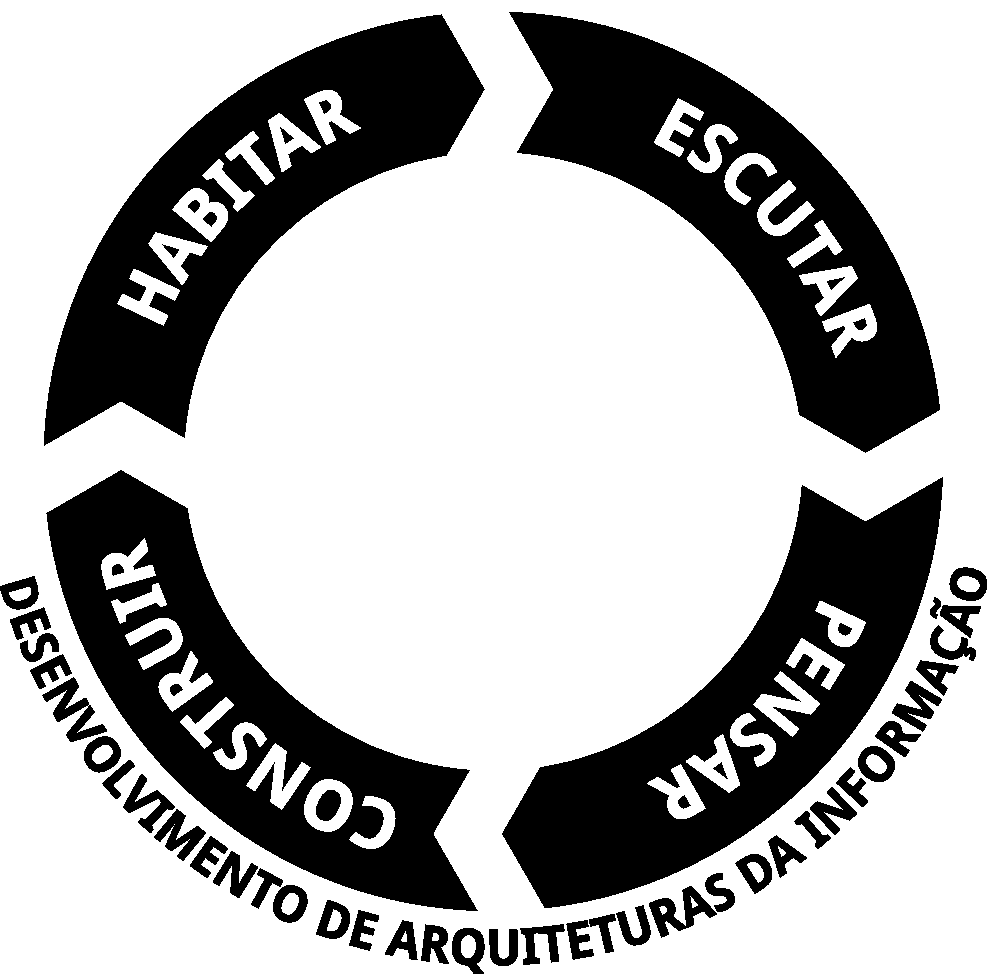
\includegraphics[width=0.4\linewidth,frame=0.5pt 5pt]{img/maia}
    \fonte{Equipe de pesquisa -- CPAI}
\end{figure}

% Texto genérico para visualizar quebra de páginas, cabeçalhos, rodapés e outros itens de formatação
\lipsum[2-3]

\lipsum[5-8]

          
          % Capítulo
            \chapter{Esse capítulo também precisa de título}\label{cap:capitulo2}
            %~~~~~~~~~~~~~~~~~~~~~~~~~~~~~~~~~~~~~~~~~~~~~~~~~~~~~~~~~~~~~~~~~~~~~
%    File      : rt_cap2
%~~~~~~~~~~~~~~~~~~~~~~~~~~~~~~~~~~~~~~~~~~~~~~~~~~~~~~~~~~~~~~~~~~~~~

Segundo capítulo do relatório. A partir desse ponto, você é livre para incluir seções, subseções e subsubseções.

\section{Essa é uma seção}\label{sec:teste}

\lipsum[2-3]

\subsection{E essa é uma subseção}\label{subsec:teste}

\lipsum[5-8]

          
          % Considerações Finais
            \chapter*[Considerações finais]{Considerações finais}\label{cap:consideracoesfinais}
            \addcontentsline{toc}{chapter}{Considerações finais}
            %~~~~~~~~~~~~~~~~~~~~~~~~~~~~~~~~~~~~~~~~~~~~~~~~~~~~~~~~~~~~~~~~~~~~~
%    File      : rt_conclusao
%~~~~~~~~~~~~~~~~~~~~~~~~~~~~~~~~~~~~~~~~~~~~~~~~~~~~~~~~~~~~~~~~~~~~~

Conclusão do relatório. Aqui você deve incluir suas observações sobre os resultados alcançados, conferir se os objetivos e metas foram cumpridos e discutir as implicações da pesquisa. Também é possível incluir aspectos sobre estudos e trabalhos futuros.

\lipsum[5-8]

          
          % Fechamento
            %~~~~~~~~~~~~~~~~~~~~~~~~~~~~~~~~~~~~~~~~~~~~~~~~~~~~~~~~~~~~~~~~~~~~~
%    File      : fechamento
%~~~~~~~~~~~~~~~~~~~~~~~~~~~~~~~~~~~~~~~~~~~~~~~~~~~~~~~~~~~~~~~~~~~~~

\begin{center}
	\rtlocal, \rtdata.
    
    \vspace{2cm}
    \rule{10cm}{0.1mm} \\
    \textsc{\rtlider} \\
    \textsc{\footnotesize Pesquisador Líder}
\end{center}

          % ------------------------------------------------------------------------------
          % - PÓS-TEXTUAL
          % ------------------------------------------------------------------------------
          \postextual          
        
          % Referências bibliográficas
            \cleardoublepage
            \bibliography{bib/rt}
        
          % Glossário
            %\glossary              % Consulte o manual da classe abntex2 para orientações sobre o glossário.

          % Apêndices
            %\part*{Apêndices}
            %\begin{apendicesenv}

                %\chapter{Título do Apêndice}\label{apend:apendice1}
                %%~~~~~~~~~~~~~~~~~~~~~~~~~~~~~~~~~~~~~~~~~~~~~~~~~~~~~~~~~~~~~~~~~~~~~
%    File      : apend01
%~~~~~~~~~~~~~~~~~~~~~~~~~~~~~~~~~~~~~~~~~~~~~~~~~~~~~~~~~~~~~~~~~~~~~

Texto do apêndice.

            %\end{apendicesenv}
                
          % Anexos
            \part*{Anexos}
            \begin{anexosenv}

                \chapter{Qual o título desse anexo?}\label{anex:anex01}
                %~~~~~~~~~~~~~~~~~~~~~~~~~~~~~~~~~~~~~~~~~~~~~~~~~~~~~~~~~~~~~~~~~~~~~
%    File      : anex01
%~~~~~~~~~~~~~~~~~~~~~~~~~~~~~~~~~~~~~~~~~~~~~~~~~~~~~~~~~~~~~~~~~~~~~

Texto do anexo.


\lipsum[2-3]

\lipsum[5-8]


            \end{anexosenv}
          
          % Índice remissimo
            \printindex

    \end{sloppypar}
\end{document}
